\newcommand\xlicho{0}
\newcommand\ylicho{7}

\newcommand\xtroj{0}
\newcommand\ytroj{4}

\newcommand\xpara{0}
\newcommand\ypara{1}

\newcommand\vyska{1.8}    % vyska
\newcommand\sirka{5}    % sirka




\begin{table}[t]
\centering
  \caption{Tvary příčných průřezů úseků hydrografické sítě a použité vztahy na výpočet hydraulického poloměru}
  \label{fig:tvary_koryt}
\begin{tabular}{p{0.4\textwidth}p{0.15\textwidth}p{0.175\textwidth}p{0.175\textwidth}}
%   \hline \\
  Tvar  & Průtočná plocha ($A$) &  Omočený obvod ($O$) & Šířka horní hrany\\ \hline
   Lichoběžník &  &  \\
  \multirow{2}{*}{
    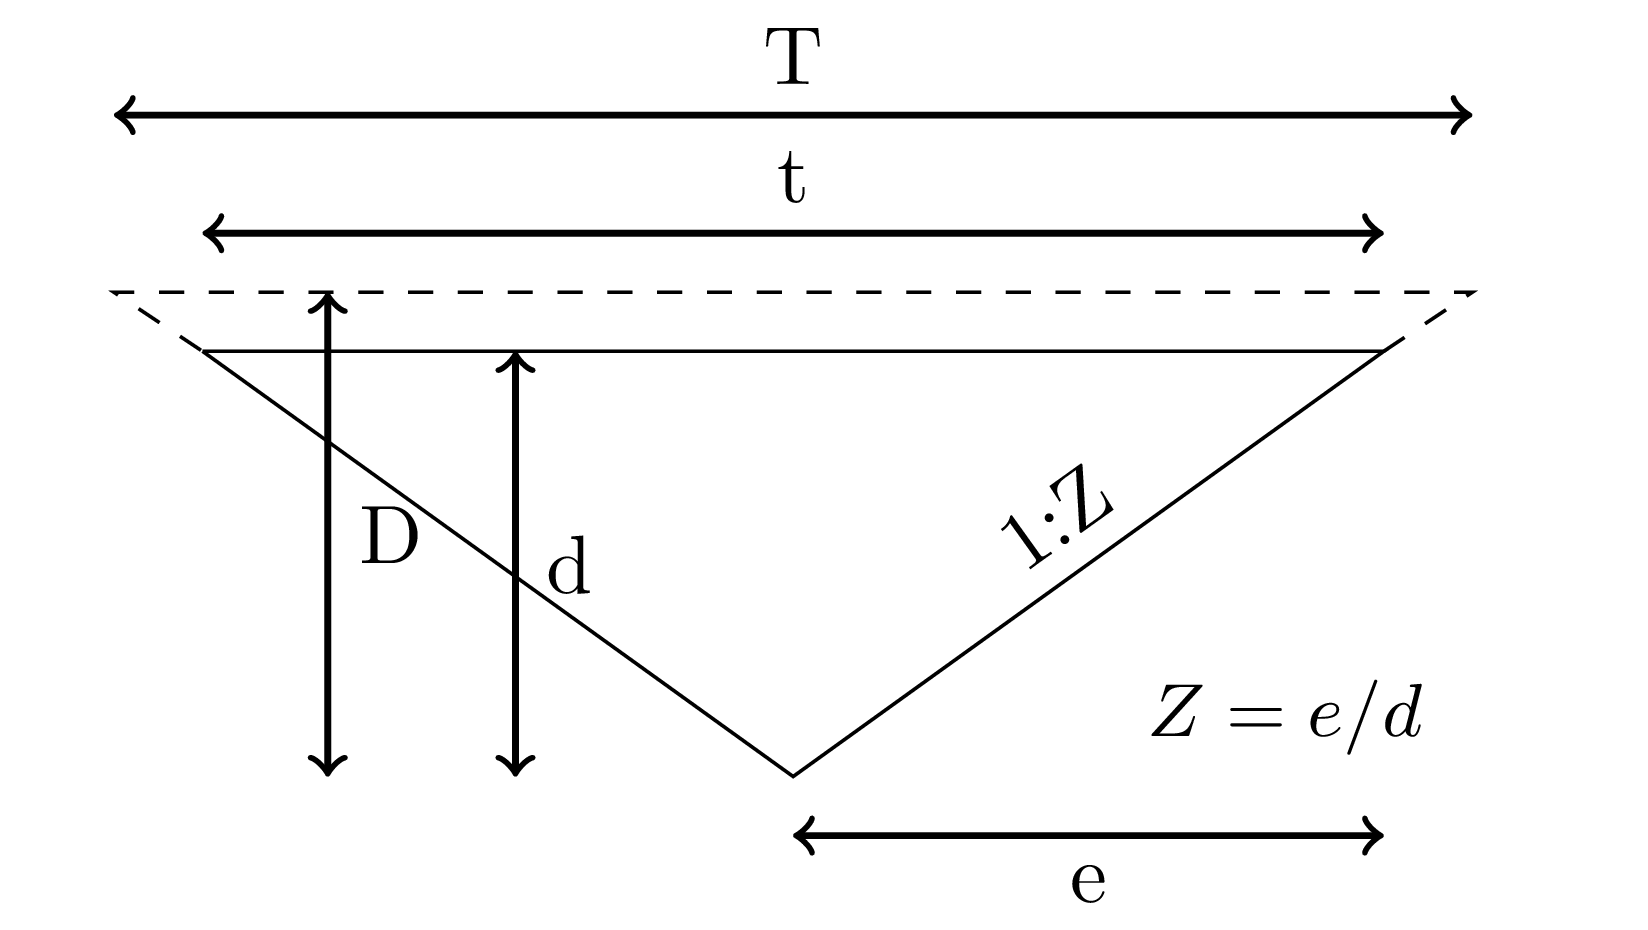
\includegraphics[width=\linewidth]{./img/trojuhelnik.png}
  } &  & & \\  
  &  &   & \\
  &  $bd + Zd^2$  & $b+2b\sqrt{1+Z^2}$  & $t = b+2dZ$ \\
  & &    & $T = b+2DZ$ \\
  &  &   & \\
  &  &  &  \\
  &  &   & \\
  &  &   & \\
%   &  &   & \\
%   &  &   & \\
  Trojúhelník &  &   & \\
 \multirow{2}{*}{
   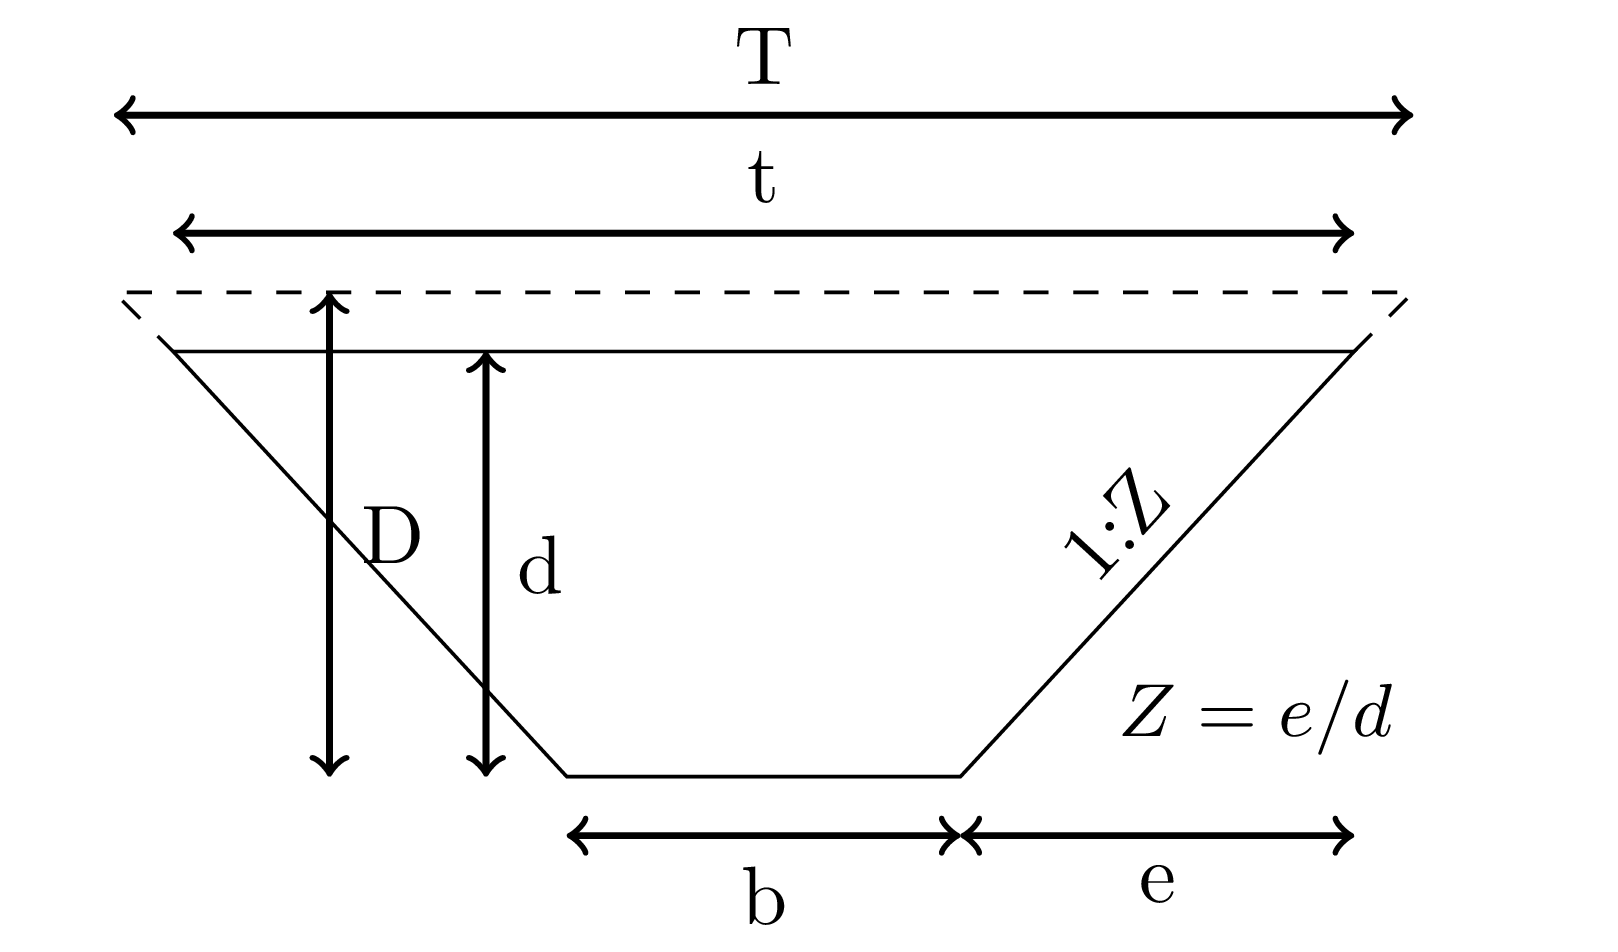
\includegraphics[width=\linewidth]{./img/lichobeznik.png}
 }   &   &   & \\
  &  &   & \\
  &  $Zd^2$   & $b+2b\sqrt{1+Z^2}$   &  $t = 2dZ$ \\
  &  &  &  $T =  2  \frac{D}{d} t$  \\
  &  &   & \\
  &  &  &  \\
  &  &  &  \\
  &  &  &  \\
%   &  &  &  \\
%   &  &  &  \\
  Parabola &  &  &  \\
 \multirow{2}{*}{
   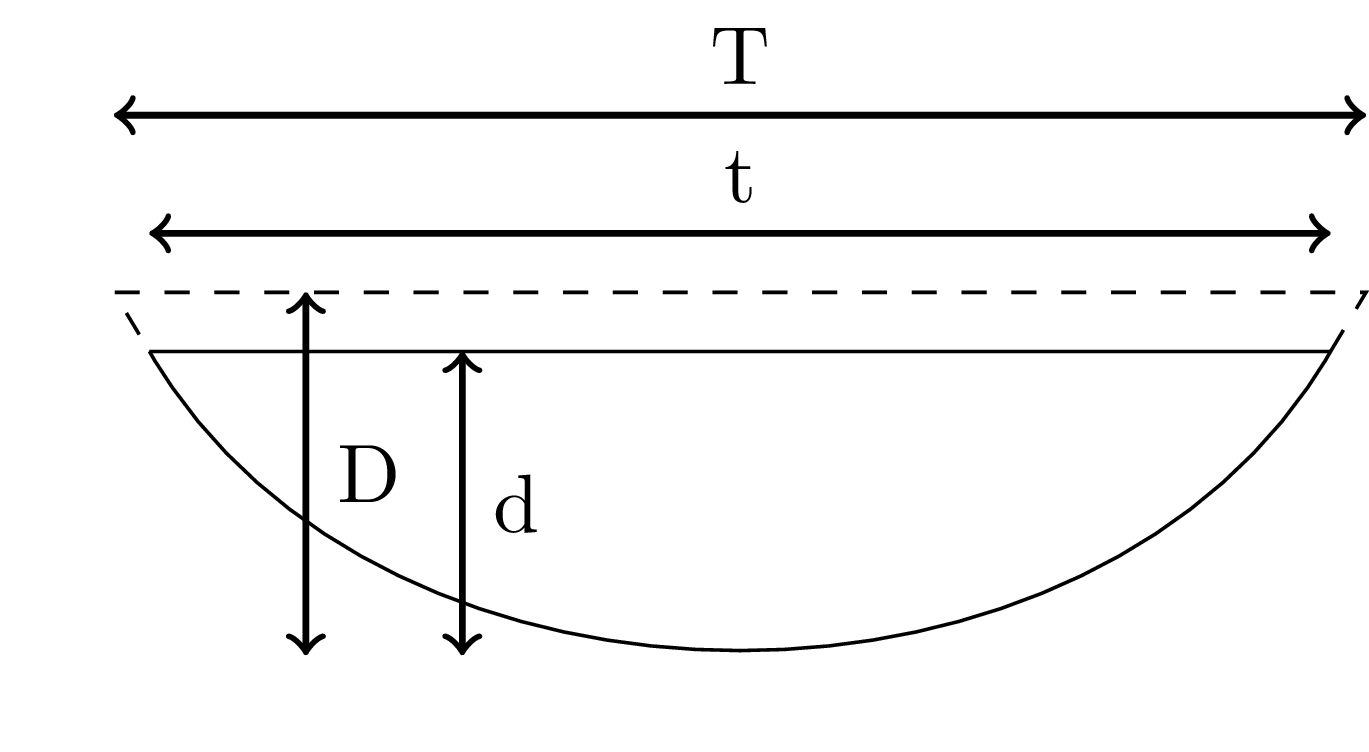
\includegraphics[width=\linewidth]{./img/parabola.png}
 }   &   &  &  \\
  &  &  &  \\
  & $\frac{2}{3}td$  & $t + \frac{8d^2}{3t} $  & $t = \frac{3A}{2d}$ \\
  &  &   &  $T = t \left(\frac{D}{d}\right)^{1/2} $ \\
  &  &   & \\
%   &  &   & \\
%   &  &   & \\
\end{tabular}
\end{table}


